\documentclass[a4paper,justified,nobib]{tufte-handout}
\usepackage{blindtext}
\usepackage{amsmath}
\usepackage{graphicx}
\usepackage{microtype}
\usepackage{biblatex}
\usepackage{tikz}

\usetikzlibrary{shapes.geometric,decorations.pathmorphing,patterns,calc}

\addbibresource{biblio.bib}

\begin{document}
\title{Resonant inductive coupling}
\author{Isawan Millican}
\maketitle

Prior to the development of the electrical grid,
there were great efforts to transmit power wirelessly by inductive coupling.
Early efforts were limited by inefficiency in transmission over larger distances.
Work carried out by Nikola Tesla in the early 20\textsuperscript{th} century
demonstrated that improved efficiency can be achieved by resonant inductive coupling.
In this article, we start by reviewing some of the key principles of electromagnetic induction.
We show how induction can be directly used to wirelessly transmit power.
This is improved by the effect of 
We then briefly consider applications of resonant inductive 


\section{A Review of Electromagnetic Induction}

Since its discovery by Faraday in 1831\cite{faradaypublishedfirst},
the phenomena of electromagnetic induction has become widely known.
The original experiment consisted of two coils of wire wrapped on opposite
sides of an iron core.
It was demonstrated that an alternating within one of the coil induces
a current in the secondary coil.
It is now known this phenomena occurs due to the generated changing magnetic
field within the soft iron core.
This phenomena forms the basis of electrical transformers and
is often highly efficient with typical efficiencies of %TODO:Efficiecy.

\begin{figure}
  \center
  %\usetikzlibrary{shapes.geometric,decorations.pathmorphing,patterns,calc}

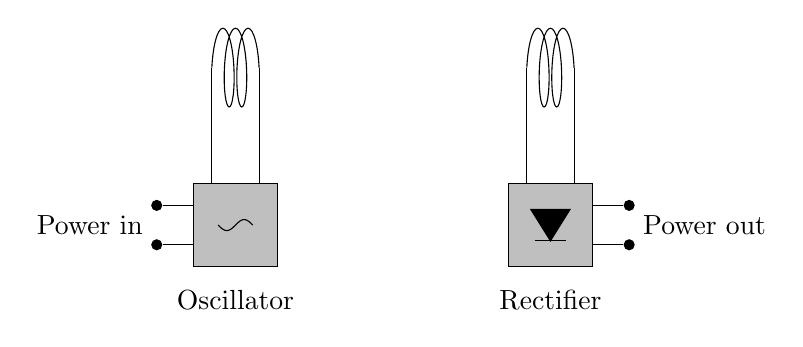
\begin{tikzpicture}[square/.style={regular polygon,regular polygon sides=4}]


% Oscillator
\node (oscillator) at (1,.25) [square,draw, minimum width=15mm,fill=lightgray]
{\tikz \draw[scale=0.07,domain=-3.141:3.141,smooth,variable=\t] plot (\t,{sin(\t r)});};
\coordinate (pcoila) at ($ (oscillator) + (-.3,2)$);
\coordinate (pcoilb) at ($ (oscillator) + (.3,2)$);
\node[circle,fill=black,inner sep=.5mm] (a) at ($(oscillator) + (-1,-0.25)$) {};
\node[circle,fill=black,inner sep=.5mm] (b) at ($(oscillator) + (-1,0.25)$) {};
\draw (a) -- (oscillator.west |- a);
\draw (b) -- (oscillator.west |- b);
\draw[decoration={aspect=0.2,segment length=1.6mm, amplitude=5mm,coil},decorate] (pcoila) -- (pcoilb);
\draw (pcoila) -- (pcoila |- oscillator.north);
\draw (pcoilb) -- (pcoilb |- oscillator.north);

% Rectifier
\node (rectifier) at (5,.25) [square,draw,minimum width=15mm,fill=lightgray] {};
\coordinate (scoila) at ($ (rectifier) + (-.3,2)$);
\coordinate (scoilb) at ($ (rectifier) + (.3,2)$);
\node[circle,fill=black,inner sep=.5mm] (c) at ($(rectifier) + (1,-0.25)$) {};
\node[circle,fill=black,inner sep=.5mm] (d) at ($(rectifier) + (1,0.25)$) {};
\draw (c) -- (rectifier.east |- c);
\draw (d) -- (rectifier.east |- d);
\draw[decoration={aspect=0.2,segment length=1.6mm, amplitude=5mm,coil},decorate] (scoila) -- (scoilb);
\draw (scoila) -- (scoila |- rectifier.north);
\draw (scoilb) -- (scoilb |- rectifier.north);
% Rectifier symbol
\coordinate (ra) at ($(rectifier)+(0,-0.2)$);
\coordinate (rb) at ($(rectifier)+(-.25,.2)$);
\coordinate (rc) at ($(rectifier)+(.25,.2)$);
\coordinate (ral) at ($(ra)+(.2,0)$);
\coordinate (rar) at ($(ra)+(-.2,0)$);
\draw (rar)--(ra)--(ral);
\draw[fill=black] (ra)--(rb)--(rc) -- cycle;

% Labels
\node at (oscillator) [below=20] {Oscillator};
\node at (oscillator) [left=30] {Power in};
\node at (rectifier) [below=20] {Rectifier};
\node at (rectifier) [right=30] {Power out};
\end{tikzpicture}

  \caption{Two coils seperated by air transfers energy by
  electromagnetic induction.
  The efficiency of this process is very low given medium seperation of the coils.}
\end{figure}

The phenomena also occurs for coils seperated by air
although the efficiency is much lower for medium seperation.
This is because the magnetic field falls $d^{-3}$ with seperation $d$
due to the magnetic field quickly diverging.
It is worth noting that reasonable efficiency can be achieved if the coils
are adjacent.
However, this is of limited usefulness.

\begin{figure}
  \center
  \usetikzlibrary{shapes.geometric,decorations.pathmorphing,patterns,calc}

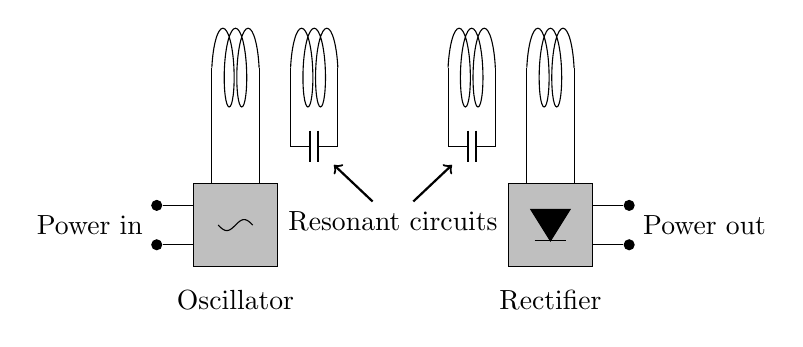
\begin{tikzpicture}[square/.style={regular polygon,regular polygon sides=4}]

% Oscillator
\node (oscillator) at (1,.25) [square,draw, minimum width=15mm,fill=lightgray]
{\tikz \draw[scale=0.07,domain=-3.141:3.141,smooth,variable=\t] plot (\t,{sin(\t r)});};
\coordinate (pcoila) at ($ (oscillator) + (-.3,2)$);
\coordinate (pcoilb) at ($ (oscillator) + (.3,2)$);
\node[circle,fill=black,inner sep=.5mm] (a) at ($(oscillator) + (-1,-0.25)$) {};
\node[circle,fill=black,inner sep=.5mm] (b) at ($(oscillator) + (-1,0.25)$) {};
\draw (a) -- (oscillator.west |- a);
\draw (b) -- (oscillator.west |- b);
\draw[decoration={aspect=0.2,segment length=1.6mm, amplitude=5mm,coil},decorate] (pcoila) -- (pcoilb);
\draw (pcoila) -- (pcoila |- oscillator.north);
\draw (pcoilb) -- (pcoilb |- oscillator.north);


% Rectifier
\node (rectifier) at (5,.25) [square,draw,minimum width=15mm,fill=lightgray] {};
\coordinate (scoila) at ($ (rectifier) + (-.3,2)$);
\coordinate (scoilb) at ($ (rectifier) + (.3,2)$);
\node[circle,fill=black,inner sep=.5mm] (c) at ($(rectifier) + (1,-0.25)$) {};
\node[circle,fill=black,inner sep=.5mm] (d) at ($(rectifier) + (1,0.25)$) {};
\draw (c) -- (rectifier.east |- c);
\draw (d) -- (rectifier.east |- d);
\draw[decoration={aspect=0.2,segment length=1.6mm, amplitude=5mm,coil},decorate] (scoila) -- (scoilb);
\draw (scoila) -- (scoila |- rectifier.north);
\draw (scoilb) -- (scoilb |- rectifier.north);
% Rectifier symbol
\coordinate (ra) at ($(rectifier)+(0,-0.2)$);
\coordinate (rb) at ($(rectifier)+(-.25,.2)$);
\coordinate (rc) at ($(rectifier)+(.25,.2)$);
\coordinate (ral) at ($(ra)+(.2,0)$);
\coordinate (rar) at ($(ra)+(-.2,0)$);
\draw (rar)--(ra)--(ral);
\draw[fill=black] (ra)--(rb)--(rc) -- cycle;


% Primary resonator
\coordinate (pcap) at (2,1.25);
\coordinate (pcapa) at ($(pcap)+(-.05,0)$);
\coordinate (pcapb) at ($(pcap)+(.05,0)$);
\coordinate (pcapcoila) at ($ (pcap) + (-.3,1)$) [circle,draw] {};
\coordinate (pcapcoilb) at ($ (pcap) + (.3,1)$) [circle,draw] {};
\draw[decoration={aspect=.2,segment length=1.6mm,amplitude=5mm,coil},decorate] (pcapcoila) -- (pcapcoilb);
\draw (pcapa) -| (pcapcoila);
\draw (pcapb) -| (pcapcoilb);
\draw[thick] ($(pcapa) +(0,.2)$) -- ($(pcapa) +(0,-.2)$);
\draw[thick] ($(pcapb) +(0,.2)$) -- ($(pcapb) +(0,-.2)$);


% Secondary resonator
\coordinate (scap) at (4,1.25);
\coordinate (scapa) at ($(scap)+(-.05,0)$);
\coordinate (scapb) at ($(scap)+(.05,0)$);
\coordinate (scapcoila) at ($ (scap) + (-.3,1)$) [circle,draw] {};
\coordinate (scapcoilb) at ($ (scap) + (.3,1)$) [circle,draw] {};
\draw[decoration={aspect=.2,segment length=1.6mm,amplitude=5mm,coil},decorate] (scapcoila) -- (scapcoilb);
\draw (scapa) -| (scapcoila);
\draw (scapb) -| (scapcoilb);
\draw[thick] ($(scapa) +(0,.2)$) -- ($(scapa) +(0,-.2)$);
\draw[thick] ($(scapb) +(0,.2)$) -- ($(scapb) +(0,-.2)$);

% Labels
\node at (oscillator) [below=20] {Oscillator};
\node at (oscillator) [left=30] {Power in};
\node at (rectifier) [below=20] {Rectifier};
\node at (rectifier) [right=30] {Power out};
\node (labelreso) at ($ (pcap)!.5!(scap) $) [below=7mm] {Resonant circuits};
\path (labelreso) edge[->,thick] ($(pcap)!.25!(labelreso)$);
\path (labelreso) edge[->,thick] ($(scap)!.25!(labelreso)$);

\end{tikzpicture}


  \caption{Diagram of an experimental apparatus demonstrating resonant inductive coupling.
    The resonant circuit is a capacitor attached to the resonating coil.
    The blue lines represent the magnetic field lines induced by the apparatus.}
    \label{fig:setupresonance}
\end{figure}

\section{Resonant inductive coupling}

The range and efficiency of the inductor can be greatly improved with electrical resonance.
The setup in figure\ref{fig:setupresonance} shows how the efficiency can be improved.
In this se







\printbibliography

\end{document}
